%Die Projektdokumentation sollte 12 bis 15 DIN A4-Seiten in üblicher Schriftgröße (z. B. Arial 10 bis 12) beinhalten.
%Zeilenabstand: 1,0 bis maximal 1,5 Zeilen
%Deckblatt mit Projekttitel und Name des Verfassers sowie Projektbetreuers, Inhaltsverzeichnis, Abbildungsverzeichnis, Glossar, Quellenverzeichnis, Kundendokumentation und Anlagen zählen nicht zu den 15 Seiten der Projektdokumentation.
%Fremde Quellen einschließlich Recherchen aus dem Internet sind deutlich zu kennzeichnen.
%Alle relevanten Inhalte der betrieblichen Projektarbeit müssen als Inhalt der Projektdokumentation vorhanden sein.
%Vertrauliche oder datenschutzrelevante Daten sind als solche zu kennzeichnen. Sofern es aus datenschutzrechtlichen Gründen erforderlich ist, können Teile der Informationen durch Schwärzen etc. unkenntlich gemacht werden.

%Uniforme Zeitform: Präteritum, muss noch umgesetzt werden: momentan noch unordentlich

\documentclass[a4paper,11pt]{report}  % Schriftgröße auf 11pt geändert
\usepackage[ngerman]{babel}
\usepackage[utf8]{inputenc}
\usepackage{geometry}
\usepackage{fancyhdr}
\usepackage{acronym}
\usepackage{glossaries}
\usepackage{setspace}
\usepackage{graphicx}
\usepackage{ragged2e}
\usepackage{lipsum}
\usepackage{hyperref}
\usepackage{tocloft}
\usepackage{array}
\usepackage{float}
\usepackage[table]{xcolor}
\usepackage{pgfgantt}
\usepackage{pdfpages}
\usepackage{csquotes}
\usepackage[T1]{fontenc}
\usepackage{titlesec} % Paket für Überschriften-Formatierung
\graphicspath{ {./img/} }

% Schriftarten Arial oder Tahoma festlegen
\usepackage{helvet}  % Für Arial
\renewcommand{\familydefault}{\sfdefault} % Sans-serif als Standard (Arial ähnlich)

% Alternativ für Tahoma, falls verfügbar:
%\usepackage{tgheros}  % Tahoma-ähnliche Schrift

\usepackage[style=numeric-comp, backend=biber, citestyle=numeric]{biblatex}

\addbibresource{literature.bib}
\makenoidxglossaries

% Layout anpassen nach DIN 5008
\geometry{a4paper, left=2.5cm, right=2cm, top=2.5cm, bottom=2cm, includeheadfoot}

% Zeilenabstand auf 1,3 setzen
\setstretch{1.3}

% Kopf- und Fußzeilen konfigurieren
\pagestyle{fancy}
\renewcommand{\chaptermark}[1]{\markboth{#1}{#1}}
\fancyhead[R]{\chaptername\ \thechapter\ --\ \chaptermark}


% Überschriften anpassen
\titleformat{\chapter}[hang]{\large\bfseries}{\thechapter}{1em}{}
\titleformat{\section}{\normalsize\bfseries}{\thesection}{1em}{}
\titleformat{\subsection}{\small\bfseries}{\thesubsection}{1em}{}

% Zeilenumbrüche verbessern

\sloppy                     % Flexible Zeilenumbrüche
\setlength{\emergencystretch}{3em}  % Erhöht Toleranz für lange Zeilen
\setlength{\headheight}{13.6pt} % Adjust header height
\addtolength{\topmargin}{-1.6pt} % Compensate for increased header height

% Acronyms und Glossaries
\newacronym{mim}{MIM}{Microsoft Identity Manager}
\newacronym{ad}{AD}{Active Directory}
\newacronym{entra}{Entra ID}{Microsoft Azure Entra ID}
\newacronym{idm}{IDM}{Identity Management}
\newacronym{sspr}{SSPR}{Self-Service-Passwortreset}
\newacronym{qs}{QS}{Qualitätssicherung}

% Definition des Kopfzeilenstils für die Verzeichnissesiten
\fancypagestyle{plain}{
    \fancyhead[R]{\chaptername\ \thechapter\ --\ \nouppercase \leftmark}
    \fancyhead[L]{\nouppercase}
    \fancyfoot[C]{\thepage}
}

\begin{document}

% Titelblatt
\begin{titlepage}
    \centering
    {
\includegraphics[width=7cm]{Projektdokumentation/img/ihk-logo.png}}\\[1em]
    {\large Abschlussprüfung Winter 2024}\\[0.5em]
    {\large Fachinformatiker für Systemintegration}\\[2em]
    {Dokumentation zur betrieblichen Projektarbeit}\\[2.5em]

    {\Large \textbf{Einführung der Self-Service-Passwortvergabe zur Ersetzung des PIN-Brief-Verfahrens bei der Erstanmeldung von Nutzern} }\\ [3em]
    {\normalsize {Abgabedatum: Frakfurt a.M., den 11.12.2024}}\\[2em]
    {\normalsize \textbf{Prüfungsbewerber:}}\\
    {\normalsize {Voller Name }}\\
    Adresse\\
    Adresse \\[2em]
    {\normalsize \textbf{Ausbildungsbetrieb: }}\\
    Firma\\
    Adresse
     Adresse \\[3em]
    {
\includegraphics[width=5cm]{Projektdokumentation/img/testing.jpg}}\\[2em]

\end{titlepage}


\includepdf[pages={1}]{persoenliche-erklaerung-data.pdf}

% Inhaltsverzeichnis 
\newpage
\pagenumbering{Roman} 
\tableofcontents

% Abbildungsverzeichnis
\newpage
\pagestyle{plain}
\addcontentsline{toc}{chapter}{Abbildungsverzeichnis}
\listoffigures

% Tabellenverzeichnis
\newpage
\pagestyle{plain}
\addcontentsline{toc}{chapter}{Tabellenverzeichnis}
\listoftables

% Abkürzungsverzeichnis
\newpage
\pagestyle{plain}
\addcontentsline{toc}{chapter}{Abkürzungsverzeichnis}
\printnoidxglossary[type=\acronymtype,title=Abkürzungsverzeichnis]

\newpage
\pagenumbering{arabic}
\setcounter{page}{1}

% Kapitel einbinden
\chapter{Einleitung}
\lipsum[1]







\chapter{Projektbeschreibung}
\lipsum[1]
\gls{mim} als auch in \gls{ad} und \gls{entra} bestehen.

\section{Projektauftrag}
\lipsum[1]

\section{Projektziele}
\subsection{Sachziel}
\lipsum[1]

\subsection{Qualitätsziel}
\lipsum[1]

\subsection{Zeitziel}
\lipsum[1]

\subsection{Kostenziel}
\lipsum[1]

\noindent \lipsum[1]

\noindent \lipsum[1]
\clearpage

\section{Projektschnittstellen und Fremdleistung}
\lipsum[1]

%Tabelle - Klarstellung von Fremdleistung und Projektschnittstellen

\begin{table}[H]
    \centering
\begin{tabular}{|  >{\centering\arraybackslash}m{7cm} | m{7cm} |}
  \hline
  \rowcolor{gray!40}
  Fachteam & Aufgabe \\
  \hline
  Identity Management Team (IDM) & Beihilfe Konfigurierung MS Azure \\
  \hline
  Identity Management Team (IDM) & Unterstützung Anpassung des Bestellformulars \\
  \hline
  Identity Management Team (IDM) & Mitwirkung bei Erstellung der Skripte \\
  \hline
  blablabla Team & Abstimmung zur Anpassung des Bestellformulars \\
  \hline
\end{tabular}
    \caption{Übersicht Fremdleistung}
    \label{tab:Übersicht Fremdleistung}
\end{table} 

\section{Mögliche Probleme}
\lipsum[1]

\section{Zeitplanung}
Die Zeitplanung erfolgt auf Basis der vorgegebenen 40 Stunden. Eine ausführliche Darstellung der Umsetzungszeiten ist im Anhang \ref{tab:Zeitplanung} \grqq{}Zeitplanung\grqq{} enthalten.




\chapter{Analyse}
In diesem Kapitel wird die aktuelle Situation analysiert und ein Zielzustand definiert.

%Diagram vorher & nachher
\section{IST-Analyse}
\lipsum[1]

\section{SOLL-Konzept}
\lipsum[1]


\section{Nutzen-Analyse}
\lipsum[1]
\chapter{Projektplanung}
Das Kapitel behandelt die Projektplanung und beschreibt die erforderlichen Werkzeuge sowie die vorbereitenden Schritte, die für die Umsetzung des Projekts notwendig sind.

\section{Terminplanung}
\lipsum[2-4]

\section{Personalplanung}
\lipsum[2-4]

\begin{table}[h!]
\centering
\begin{tabular}{|l|l|l|l|}
\hline
\textbf{Team} & \textbf{Name} & \textbf{Tätigkeit} &  \textbf{Stunden}  \\ \hline
IDM        & name      & Projektumsetzung & 40       \\ \hline
IDM        & name    & Ansprechpartner, Projektübergabe & 8        \\ \hline
IDM        & name          & Projektdefinition, Projektunterstützung & 8        \\ \hline
IDM        & name                & Projektunterstützung                      & 8         \\ \hline
\end{tabular}
\caption{Personalplanung}
\label{tab:Personalplanung}
\end{table}

\section{Sachmittelplanung}
Die für das Projekt benötigten Materialien sind bereits verfügbar und müssen nicht extra angeschafft werden.
%nachfrage

\begin{longtable}{|l|p{10cm}|}
\hline
\textbf{Sachmittel}         & \textbf{Beschreibung}                                            \\ \hline
PC-Arbeitsplatz             & Umsetzung und Realisierung des Projektes sowie der Kommunikation \\ \hline
Microsoft Windows 10        & Betriebssystem für den Arbeitsplatz-PC                           \\ \hline
Microsoft Word              & Erstellen von Dokumenten und Anleitungen                         \\ \hline
Microsoft Teams             & Kommunikation zwischen Kollegen                                  \\ \hline
Microsoft Outlook           & Senden von Mails                                                 \\ \hline
Microsoft Azure/Entra       & Administrationsschnittstelle für Nutzerverwaltung                \\ \hline
Microsoft Edge              & gewählter Browser zur Bearbeitung der Konfigurationen            \\ \hline
Overleaf                    & Erstellung der Projektdokumentation in \LaTeX                    \\ \hline
\caption{Sachmittelplanung} \\
\end{longtable}

\section{Kostenplanung}
Die Kostenplanung erfolgt unter Berücksichtigung von Personal- und Lizenzkosten, wobei für die Berechnung der Personalkosten fiktive Stundensätze herangezogen werden, die sowohl die Löhne als auch die Lohnkosten sowie die Sachkosten umfassen.

\begin{table}[h!]
\centering
\begin{tabular}{|l|l|c|l|}
\hline
\textbf{Mitarbeiter} & \textbf{Stunden} & \textbf{Stundensatz} & \textbf{Gesamtkosten} \\ \hline
name   & 40     & 100€         & 4.000,00€   \\ \hline
name & 8      & 150€         & 1.200,00€   \\ \hline
name     & 8      & 150€         & 1.200,00€   \\ \hline
name            & 8      & 150€         & 1.200,00€   \\ \hline
Gesamt                 &        &              & 7.600,00€   \\ \hline
\end{tabular}
\caption{Personalkosten}
\label{tab:Personalkosten}
\end{table}


\section {Schutzbedarfsanalyse}
\lipsum[1]
\chapter{Realisierung}
\lipsum[1]

\section{Proof of Concept}
\lipsum[1]



\section{Entra-SSPR-Konfiguration}
\lipsum[1]

\section{Anpassung Bestellformulars}
\lipsum[1]

\section{Erstellung des Fufillment Prozesses} 
\lipsum[1]

\subsection{Lifecycleprozesse} \label{Lifecycleprozess}
Der Benutzer Account Lifecycle \footnote{\cite[Was ist der User Account Lifecycle?]{lifecycle}}
\lipsum[1]

\section{Ablauf der Passwort Vergabe}
\lipsum[1]

\section{Produktivnahme/Staging}
\lipsum[1]

\chapter{Projektabschluss}
\lipsum[1]

\section{SOLL / IST Vergleich}
\lipsum[1]

\subsection{Sachziel}
\lipsum[1]

\subsection{Qualitätsziel}
%Zusammenfassung der Realisierung
Die \acrshort{sspr}-Konfiguration wurde erfolgreich eingerichtet. 
\lipsum[1]

\subsection{Zeitziel}
Das Projekt wurde innerhalb des vorgesehenen Zeitrahmens abgeschlossen, und die Bearbeitungszeit von 40 Stunden wurde eingehalten. Während des Projekts war es notwendig, den Zeitplan anzupassen. Eine Übersicht der geplanten und tatsächlichen Zeiten ist im Anhang \grqq{}\ref{tab:Vergleich Zeitplanung}\grqq{} zu finden.

%\ref{fig:Vergleich Zeitplanung} 


\subsection{Kostenziel}
\lipsum[1]

\section{Ausblick}
\lipsum[1]

\section{Reflektion}
\lipsum[1]

\section{Fazit}
\lipsum[1]
\clearpage



\newpage
\pagenumbering{Roman} 
\setcounter{page}{6}
\chapter{Anlagenverzeichnis}

\section{Zeitplanung}
\begin{table}[h!]
    \centering
\begin{tabular}{|  >{\columncolor{gray!40}\centering\arraybackslash}m{0.5cm} | m{11cm} | >{\centering\arraybackslash}m{3cm} |}
  \hline
  \rowcolor{gray!40}
  Nr. & Aufgabe & Zeitansatz [h] \\
  \hline
  \rowcolor{gray!20}
  & Analyse & 3 \\
  \hline
  1 & IST-Analyse & 1 \\
  \hline
  2 & Nutzenanalyse & 1 \\
  \hline
  3 & Schutzbedarfsanalyse & 1 \\
  \hline
  \rowcolor{gray!20}
  & Planung & 3 \\
  \hline
  4 & Proof of Concept & 3 \\
  \hline
  \rowcolor{gray!20}
  & Realisierung & 11 \\
  \hline
  5 & Entra-SSPR-Konfiguration & 3 \\
  \hline
  6 & Anpassung des Bestellformulars & 2 \\
  \hline
  7 & Erstellung des Fulfillment Prozesses & 6 \\
  \hline
  \rowcolor{gray!20}
  & Produktivnahme & 12 \\
  \hline
  8 & Benutzerdoku erstellen & 3 \\
  \hline
  9 & Lifecycleprozesse & 3 \\
  \hline
  10 & Stageing & 6 \\
  \hline
  \rowcolor{gray!20}
  & Abschluss & 10 \\
  \hline
  11 & IST-SOLL-Vergleich & 1 \\
  \hline
  13 & Dokumentation erstellen & 9 \\
  \hline
  \rowcolor{gray!60}
   & Summe & 40 \\
  \hline
\end{tabular}
    \caption{Zeitplanung}
    \label{tab:Zeitplanung}
\end{table}



\begin{figure}[H]
\section{Projektlaufzeit}
    \centering
    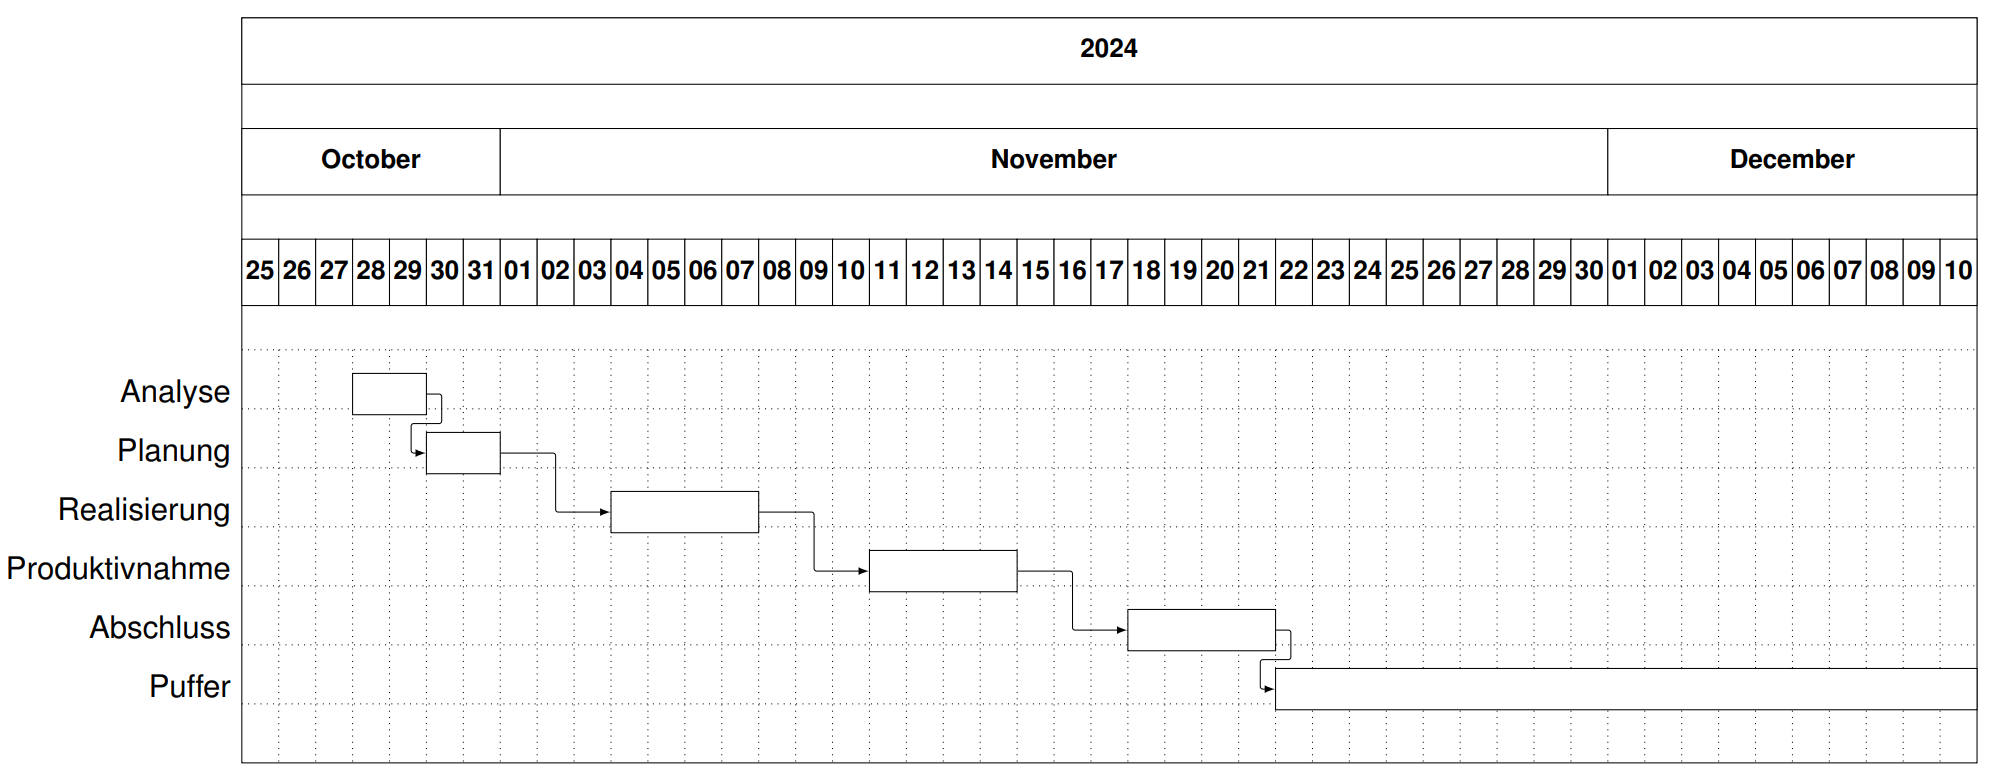
\includegraphics[width=1.0\textwidth]{Projektdokumentation/img/Projektlaufzeit.png}
    \caption{Projektlaufzeit}
    \label{fig:Projektlaufzeit}
\end{figure}

\section{Schutzbedarfsanalyse}
\begin{table}[H]
\centering
\begin{tabular}{|l|c|c|c|c|}
\hline
\textbf{ }          & \textbf{Vertraulichkeit} & \textbf{Integrität} & \textbf{Verfügbarkeit} & \textbf{Schutzbedarf gesamt} \\ \hline
MIM                         & Hoch                    & Mittel              & Hoch                   & Hoch                         \\ \hline
Verfügbarkeit der Daten     & Niedrig                 & Mittel              & Hoch                   & Mittel                       \\ \hline
\end{tabular}
\caption{Schutzbedarfsanalyse}
\label{tab:schutzbedarfsanalyse}
\end{table}

\begin{figure}[H]
\section{Authentifkationsmethoden}
    \centering
    
\includegraphics[width=1.0\textwidth]{Projektdokumentation/img/testing.jpg}
    \caption{Authentifkationsmethoden}
    \label{fig:Authentifkationsmethoden}
\end{figure}

\begin{figure}[H]
\section{SSPR-Gruppe}
    \centering
    
\includegraphics[width=1.0\textwidth]{Projektdokumentation/img/testing.jpg}
    \caption{SSPR-Gruppe}
    \label{fig:SSPR-Gruppe}
\end{figure}

\section{Bestellformular für einen externen Benutzer}
\begin{figure}[H]
    \centering
    
\includegraphics[width=1\textwidth]{Projektdokumentation/img/testing.jpg}
    \caption{Bestellformular}
    \label{fig:Bestellformular}
\end{figure}


\begin{figure}[H]
\section{Audit Logs}
    \centering
    
\includegraphics[width=1.0\textwidth]{Projektdokumentation/img/testing.jpg}
    \caption{Audit Logs}
    \label{fig:Audit Logs}
\end{figure}


\section{Vergleich Zeitplanung}

\begin{table}[H]
    \centering
\begin{tabular}{|  >{\columncolor{gray!40}\centering\arraybackslash}m{0.5cm} | m{6.5cm} | >{\centering\arraybackslash}m{3.5cm} | >{\centering\arraybackslash}m{3.5cm} |}
  \hline
  \rowcolor{gray!40}
  Nr. & Aufgabe & Zeitansatz [h] & Benötigt [h] \\
  \hline
  \rowcolor{gray!20}
  & Analyse & 3 &3\\
  \hline
  1 & IST-Analyse &\cellcolor{yellow!25} 1 &\cellcolor{yellow!25} 1 \\
  \hline
  2 & Nutzenanalyse &\cellcolor{yellow!25} 1 &\cellcolor{yellow!25} 1 \\
  \hline
  3 & Schutzbedarfsanalyse &\cellcolor{yellow!25} 1 &\cellcolor{yellow!25}1 \\
  \hline
  \rowcolor{gray!20}
  & Planung & 3 & 3\\
  \hline
  4 & Proof of Concept &\cellcolor{yellow!25} 3 &\cellcolor{yellow!25} 3 \\
  \hline
  \rowcolor{gray!20}
  & Realisierung & 11 & 11 \\
  \hline
  5 & Entra-SSPR-Konfiguration &\cellcolor{blue!25} 3 &\cellcolor{blue!25} 2 \\
  \hline
  6 & Anpassung des Bestellformulars &\cellcolor{blue!25} 2 &\cellcolor{blue!25} 4 \\
  \hline
  7 & Erstellung des Fulfillment Prozesses &\cellcolor{blue!25} 6 &\cellcolor{blue!25} 5 \\
  \hline
  \rowcolor{gray!20}
  & Produktivnahme & 12 & 12 \\
  \hline
  8 & Benutzerdoku erstellen &\cellcolor{yellow!25} 3 &\cellcolor{yellow!25} 3 \\
  \hline
  9 & Lifecycleprozesse &\cellcolor{yellow!25} 3 &\cellcolor{yellow!25} 3\\
  \hline
  10 & Staging &\cellcolor{yellow!25} 6 &\cellcolor{yellow!25} 6\\
  \hline
  \rowcolor{gray!20}
  & Abschluss & 10 & 10\\
  \hline
  11 & IST-SOLL-Vergleich &\cellcolor{blue!25} 1 &\cellcolor{blue!25} 2 \\
  \hline
  13 & Dokumentation erstellen &\cellcolor{blue!25} 9 &\cellcolor{blue!25} 8 \\
  \hline
  \rowcolor{gray!60}
   & Summe & 40 & 40\\
  \hline
\end{tabular}
    \caption{Vergleich Zeitplanung}
    \label{tab:Vergleich Zeitplanung}
\end{table}








% Nummerierung in Buchstaben ändern
\setcounter{chapter}{0} % Kapitelzähler zurücksetzen
\renewcommand{\thechapter}{\Alph{chapter}}

% Literaturverzeichnis
\newpage
\pagestyle{plain}
\addcontentsline{toc}{chapter}{Literaturverzeichnis}
\printbibliography

\end{document}